\section{Flywheel brake study}

This section aims to study a possible way to break the flywheel without applying torque to the platform. The idea is combining both methods:
we will leave the moving weight free.

This way, when the weight is going upward will have a larger radius than when is going downward and will produce an average moment against the movement of the flywheel.

From an energetic point of view we are transforming the rotation energy of the flywheel in to translation of the free cylinder and then realising it trough collisions.
\subsection{System of differential equations}
As described in figure \ref{fig:Flywheel force diagram} we will use two variables to describe the flywheel position: $r$, $\theta$ 

Using equation \ref{eq: flywheel torque equation}:
\[\tau_{motor-flywheel} = \ddot{\theta}*I_{flywheel}(r) + m_{cylinder} * g * 
(r_{max} - r) * \sin({\theta})  \]
\begin{figure}[H]
	\centering
	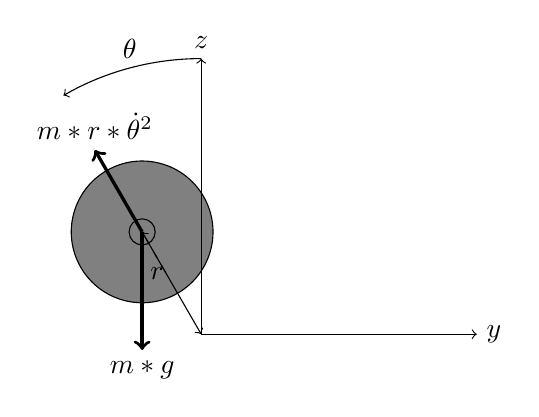
\begin{tikzpicture}
        %Center
            \path node (center) at (0,0) {};
        %Arcs
            \draw[->] (0,3.5) arc (90:120:3.5) node[above, midway]{$\theta$};
        %Movable mass
            \draw[rotate=120,fill=gray] (1.5,0) circle (.9) node (moving) [draw,circle]{};
        %Guide
            \draw[dashed,rotate=120] (.9,0) -- (2.1,0);
        %Radius
            \draw[<->] (0,0) -- (moving.center) node[near end, below] {$r$};
		%Forces
			\draw[->, very thick] (moving.center) -- ([shift=({0,-1.5})]moving.center) node[below]{$m*g$};
			\draw[->, very thick, rotate=120] (1.5,0) -- (2.7,0) node[above]{$m*r*\dot{\theta}^2$};
		%Axis
            \draw[->,thin] (center.center) -- (0,3.5) node[above] {$z$};
            \draw[->,thin] (center.center) -- (3.5,0) node[right] {$y$};
    \end{tikzpicture}
	\caption{Cylinder force diagram}
	\label{fig:Cylinder force diagram}
\end{figure}

As seen in figure \ref{fig:Cylinder force diagram}, we can deduce newtons equation for the distance from the cylinder to the center $r$. Note that we are adding the centrifugal force term due to the non-inertial frame.
\[\ddot{r} * m = -m * g * cos(\theta) + m * r * \dot{\theta}^2 \]
\[\ddot{r} = -g * cos(\theta) + r * \dot{\theta}^2 \]

The variables we will be using for our ODE system are: $r$,$\dot{r}$,$\theta$,$\dot{\theta}$

Note that we impose $\tau_{flywheel} = 0$ so the motor is not applying any torque.

\[
\begin{cases}
    \dot{r} = \dot{r}\\
    \ddot{r} = -g * cos(\theta) + r * \dot{\theta}^2\\
    \dot{\theta} = \dot{\theta}\\
    \ddot{\theta} = \frac{m_{cylinder} * g * (r - r_{max}) * \sin{\theta}}{I_{flywheel}(r)} \\    
\end{cases}
\]


Our initial conditions will be the free cylinder mass lying on the bottom of the flywheel and the flywheel turning at a speed $\theta_0$:
\[
    \begin{cases}
        r = r_{max} \\
        \dot{r} = 0\\
        \theta = \pi\\
        \dot{\theta} = \theta_0\\
    \end{cases}
\]

We will use a poincare map to simulate the bounce with the end of the guides at $r=r_{min}$ and $r=r_{max}$. At each bounce we will reduce its kinetic energy by a percentage $bounce\_percentage$ .

\subsection{Results}
The parameters of the simulation where:
\[
\begin{cases}
	r_{flywheel} = 8cm \\
	r_{wheel} = 9cm \\
	w = 7 cm \\
	\dot{\theta}_0 = 4.2 \pi rad/s \\
	bounce\_percentage = 0.0 (totally inelastic) \\	
\end{cases}	
\]

\begin{figure}[H]
	\centering
	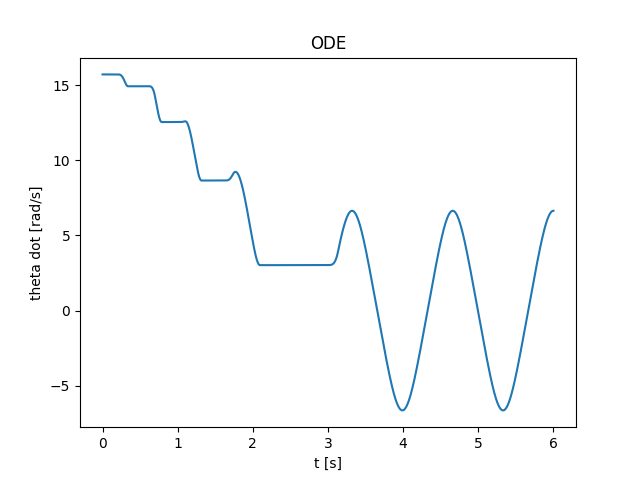
\includegraphics[width=10cm]{img/simulation/d_theta_t.png}
	\caption{How the variable $\dot{\theta}$ evolve over time}
	\label{fig:d theta t diagram}
\end{figure}
As we can see in figure \ref{fig:d theta t diagram} the flywheel is braking until it becomes a pendulum and starts oscillating.

\begin{figure}[H]
	\centering
	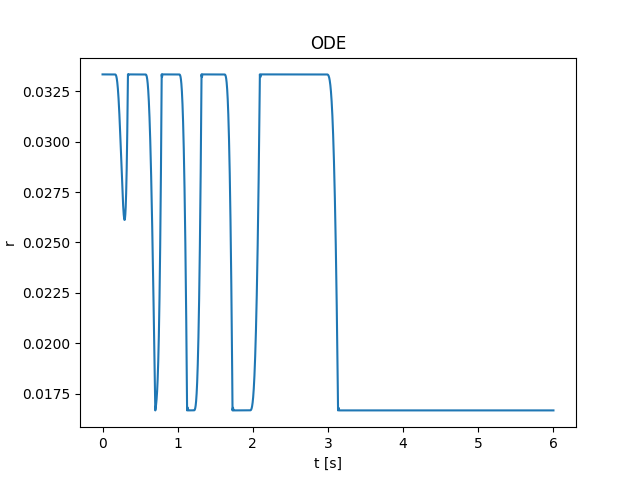
\includegraphics[width=10cm]{img/simulation/r_t.png}
	\caption{How the variable $r$ evolves over time}
	\label{fig:r t diagram}
\end{figure}
In the first laps the cylinder is almost always at the maximum value of r, but as the
speed decrease each lap the value of $r$ decrease until it hits the $r_{min}$.
In other words, at the begining is operating as a flywheel but then thanks to the
collisions it becomes a pendulum.

\begin{figure}[H]
	\centering
	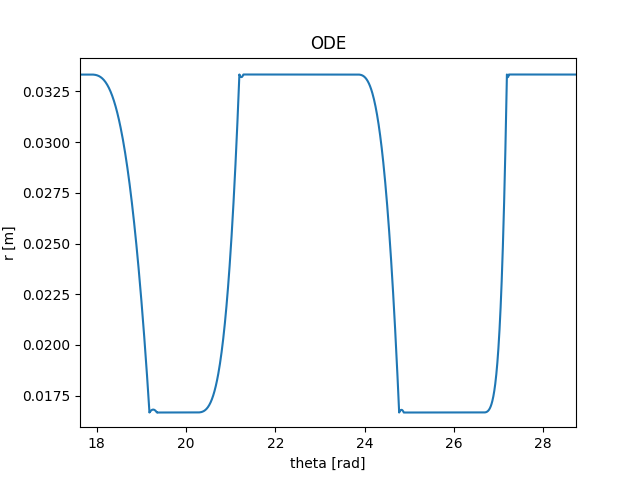
\includegraphics[width=10cm]{img/simulation/r_theta_t_zoom.png}
	\caption{How the variable $r$ evolve over $\theta$ zoomed}
	\label{fig:r theta zoom}
\end{figure}
In image \ref{fig:r theta zoom} we can appreciate that the r decrease slower that what it increase.


\begin{figure}[H]
	\centering
	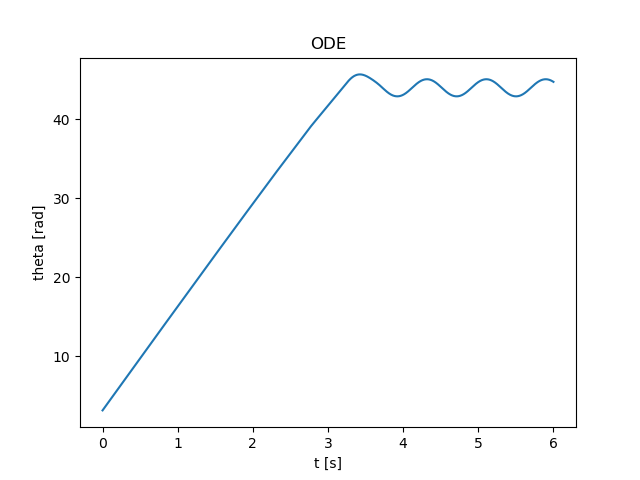
\includegraphics[width=10cm]{img/simulation/theta_t.png}
	\caption{How the variable $\theta$ evolves over time}
	\label{fig:theta t diagram}
\end{figure}

\begin{figure}[H]
	\centering
	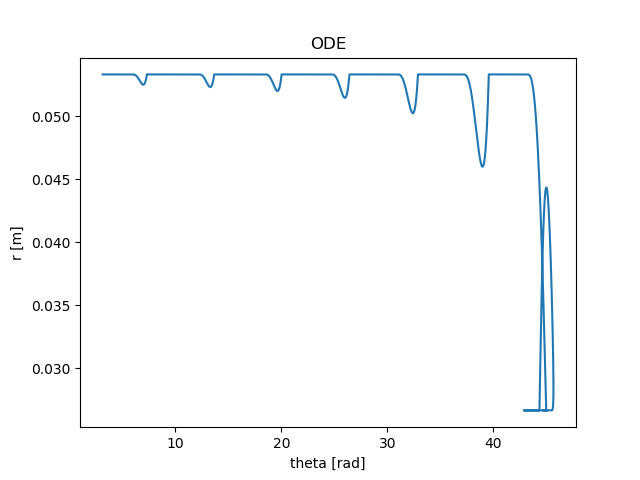
\includegraphics[width=10cm]{img/simulation/r_theta_t.png}
	\caption{How the variable $r$ evolves over $\theta$}
	\label{fig:r theta}
\end{figure}

